\documentclass[12pt,a4paper]{article}
\usepackage[utf8]{inputenc}
\usepackage[T1]{fontenc}
\usepackage[spanish,es-tabla]{babel}
\usepackage{graphicx}
\usepackage{float}
\usepackage{geometry}
\usepackage{hyperref}
\usepackage{fancyhdr}
\usepackage{titlesec}
\usepackage{booktabs}
\usepackage{array}
\usepackage{longtable}
\usepackage[table]{xcolor}
\usepackage{mathptmx}
\usepackage{amsmath}
\usepackage{enumitem}
\setlist{itemsep=0pt,topsep=2pt,parsep=0pt}
\setlength{\belowcaptionskip}{4pt}
\renewcommand{\topfraction}{0.9}
\renewcommand{\bottomfraction}{0.8}
\renewcommand{\textfraction}{0.1}
\renewcommand{\floatpagefraction}{0.7}
\setcounter{topnumber}{3}
\setcounter{totalnumber}{5}
\usepackage{setspace}
\usepackage{xurl}
\usepackage{verbatim}

\geometry{top=2.5cm, bottom=2.5cm, left=3cm, right=3cm}
\hypersetup{colorlinks=true, linkcolor=black, urlcolor=blue, citecolor=black}
\graphicspath{{data/}{outputs/figuras/}}

% bloque "Cómo leerla" de figuras y tablas de resultados
\newcommand{\comoleerla}[3]{%
  \begin{center}\footnotesize
  \begin{minipage}{0.94\linewidth}
  \begin{itemize}\setlength{\itemsep}{0pt}\setlength{\topsep}{2pt}%
    \setlength{\parsep}{0pt}
  \item \textbf{Estructura:} #1
  \item \textbf{Qué se ve:} #2
  \item \textbf{Por qué:} #3
  \end{itemize}
  \end{minipage}
  \end{center}}

% cifras del informe, generadas por informe/tablas_corte3.py
% Generado por informe/tablas_corte3.py: no editar a mano.
\newcommand{\ctFilasCrudas}{149\,944}
\newcommand{\ctPeajesCrudos}{162}
\newcommand{\ctCategorias}{55}
\newcommand{\ctPrimerMes}{enero de 2014}
\newcommand{\ctUltimoMes}{mayo de 2026}
\newcommand{\ctFilasSinClase}{23\,300}
\newcommand{\ctTransitoSinClase}{0.27}
\newcommand{\ctPctLivianos}{67.2}
\newcommand{\ctPctBuses}{14.1}
\newcommand{\ctPctCarga}{17.8}
\newcommand{\ctPctUnica}{0.8}
\newcommand{\ctFilasPeajeMes}{16\,779}
\newcommand{\ctMesesSinTransito}{32}
\newcommand{\ctMesesAnomalos}{25}
\newcommand{\ctMesesParciales}{57}
\newcommand{\ctUmbralAnomalo}{10}
\newcommand{\ctUmbralParcial}{50}
\newcommand{\ctFilasDepuradas}{16\,665}
\newcommand{\ctFilasModelables}{14\,297}
\newcommand{\ctPeajesModelables}{158}
\newcommand{\ctTransitoMediano}{4\,600}
\newcommand{\ctTransitoMaximo}{42\,466}
\newcommand{\ctMesMinimo}{abril de 2020}
\newcommand{\ctCaidaMinimo}{68}
\newcommand{\ctCorteBajo}{3\,284}
\newcommand{\ctCorteAlto}{6\,564}
\newcommand{\ctFilasEntrenamiento}{11\,348}
\newcommand{\ctFilasValidacion}{1\,486}
\newcommand{\ctFilasPrueba}{1\,463}
\newcommand{\ctPeajesPrueba}{125}
\newcommand{\ctMejorRegresor}{Bosque aleatorio}
\newcommand{\ctMaeMejor}{358.8}
\newcommand{\ctRmseMejor}{669.3}
\newcommand{\ctRdosMejor}{0.9880}
\newcommand{\ctEpmMejor}{3.94}
\newcommand{\ctMaePersistencia}{554.4}
\newcommand{\ctMaeEstacional}{605.6}
\newcommand{\ctEpmPersistencia}{5.97}
\newcommand{\ctMejoraMae}{35}
\newcommand{\ctMaeLineal}{419.9}
\newcommand{\ctMaeArbol}{476.5}
\newcommand{\ctPrimeraVariable}{tránsito del mes anterior}
\newcommand{\ctPrimeraImportancia}{0.540}
\newcommand{\ctSegundaVariable}{tránsito de hace 2 meses}
\newcommand{\ctSegundaImportancia}{0.071}
\newcommand{\ctHorizonteUno}{4.5}
\newcommand{\ctHorizonteDoce}{6.2}
\newcommand{\ctHorizonteMaximo}{7.4}
\newcommand{\ctHorizontesGana}{7}
\newcommand{\ctEstacionalDoce}{7.1}
\newcommand{\ctPersistenciaMaxima}{18.6}
\newcommand{\ctMejorClasificador}{Bosque aleatorio}
\newcommand{\ctExactitudMejor}{94.53}
\newcommand{\ctFunoMejor}{94.57}
\newcommand{\ctExactitudPersistencia}{91.39}
\newcommand{\ctExactitudDerivada}{94.19}
\newcommand{\ctErroresClasificacion}{80}
\newcommand{\ctErroresExtremos}{0}
\newcommand{\ctPeajesAgrupados}{148}
\newcommand{\ctKGrupos}{4}
\newcommand{\ctSiluetaKmedias}{0.270}
\newcommand{\ctSiluetaJerarquico}{0.254}
\newcommand{\ctRandAjustado}{0.77}
\newcommand{\ctVarianzaPlano}{65}
\newcommand{\ctGrupoMayor}{1}
\newcommand{\ctGrupoMayorTransito}{11\,087}
\newcommand{\ctGrupoMayorEnRed}{10}
\newcommand{\ctGrupoEstacional}{4}
\newcommand{\ctGrupoEstacionalAmplitud}{0.71}
\newcommand{\ctTramosVigentes}{14}
\newcommand{\ctTramosHistoricos}{7}
\newcommand{\ctTramosSinDato}{11}
\newcommand{\ctTramosConPeaje}{24}
\newcommand{\ctTramosConSerie}{21}
\newcommand{\ctTramosDobleCalzada}{8}
\newcommand{\ctFilasTramoMes}{2\,450}
\newcommand{\ctSaturacionMediana}{0.18}
\newcommand{\ctSaturacionMaxima}{0.67}
\newcommand{\ctFactorMaximo}{1.0303}
\newcommand{\ctDemoraMaxima}{2.07}
\newcommand{\ctTramoDemoraMaxima}{Chocontá - Tunja}
\newcommand{\ctMesDemoraMaxima}{diciembre de 2025}
\newcommand{\ctCasosTiempo}{162}
\newcommand{\ctMaeTiempo}{0.019}
\newcommand{\ctErrorMaximoTiempo}{0.74}
\newcommand{\ctMesEjemplo}{diciembre de 2026}
\newcommand{\ctCasoKm}{370.54}
\newcommand{\ctCasoTiempo}{7 h 27 min}
\newcommand{\ctCasoLibre}{7 h 25 min}
\newcommand{\ctCasoDemora}{1.84}
\newcommand{\ctCasoAlto}{4}
\newcommand{\ctCasoSinDato}{2}
\newcommand{\ctCasoTramos}{8}
\newcommand{\ctCasoExpandidos}{14}
\newcommand{\ctCasoReexpansiones}{0}
\newcommand{\ctAlternativaKm}{654.25}
\newcommand{\ctAlternativaTiempo}{13 h 05 min}
\newcommand{\ctAlternativaAlto}{0}
\newcommand{\ctAlternativaMas}{339}
\newcommand{\ctDemoraMinimaCaso}{0.41}
\newcommand{\ctDemoraMaximaCaso}{1.84}
\newcommand{\ctVelocidadLibre}{50}


\pagestyle{fancy}
\fancyhf{}
\fancyhead[L]{\small Corte 3: aprendizaje automático e integración}
\fancyhead[R]{\thepage}
\renewcommand{\headrulewidth}{0.4pt}
\setlength{\headheight}{14.5pt}
\setlength{\emergencystretch}{3em}

\titleformat{\section}{\normalfont\Large\bfseries}{\thesection}{1em}{}
\titleformat{\subsection}{\normalfont\large\bfseries}{\thesubsection}{1em}{}

\begin{document}

\begin{titlepage}
\thispagestyle{empty}
\centering

\vspace*{0.5cm}

\includegraphics[width=0.30\textwidth]{sergio_logo.png}\\[0.4cm]

{\fontsize{13}{15}\selectfont\textbf{UNIVERSIDAD SERGIO ARBOLEDA}}\\[2.0cm]

{\fontsize{14}{17}\selectfont\textbf{APRENDIZAJE AUTOMÁTICO E INTEGRACIÓN EN UNA\\
RED DE CARGA INTERURBANA: REGRESIÓN,\\
CLASIFICACIÓN Y AGRUPAMIENTO DEL TRÁNSITO}}\\[0.6cm]
{\fontsize{12}{14}\selectfont Proyecto Integrador, Corte 3 (informe final)}\\[2.2cm]

{\fontsize{12}{14}\selectfont\textbf{Inteligencia Artificial (SIST5036)}}\\[1.5cm]

{\fontsize{12}{14}\selectfont
Juan David Andradé Gómez\\[0.2cm]
Mario Jiménez López\\[0.2cm]
Camilo Andrés Díaz García}\\[1.2cm]

{\fontsize{12}{14}\selectfont Profesor: Joaquín F. Sánchez}

\vfill

\begin{center}
    \textit{Universidad Sergio Arboleda}\\
    \textit{Facultad de Sistemas e Ingeniería}\\
    \textit{Bogotá D.C., 2026}
\end{center}

\end{titlepage}

\newpage
\tableofcontents
\newpage

\section{Alcance y continuidad}
\label{sec:alcance}

El Corte 1 formuló el problema y construyó la red de 32 nodos y 32
aristas~\cite{formulacion}. El Corte 2 implementó y comparó los cinco
algoritmos de búsqueda sobre esa red~\cite{cortedos}. Este corte agrega los
tres modelos de aprendizaje automático que pide el proyecto y los integra con
el agente y con la aplicación web.

\textbf{Qué pide el corte y cómo se resolvió.}
\begin{itemize}
\item \textbf{Regresión del tiempo de desplazamiento.} Se predice el tránsito
diario de cada peaje y, con él, el tiempo de recorrido de cada tramo.
\item \textbf{Clasificación de la congestión.} Se predice el nivel de
tránsito del mes: bajo, medio o alto.
\item \textbf{Agrupamiento.} Se agrupan los peajes por su perfil de tránsito
con K-medias y con agrupamiento jerárquico.
\item \textbf{Integración.} Un agente predictivo usa los pronósticos para
buscar con A* la ruta de menor tiempo estimado, y la aplicación web lo
muestra sobre el mapa.
\end{itemize}

\textbf{Limitación de partida.} Los datos de los cortes anteriores (INVÍAS y
ANSV) traen distancia, peaje y riesgo. No traen tiempos, velocidades ni
congestión. Se tomaron dos decisiones:
\begin{itemize}
\item \textbf{Dato real de tránsito.} Se incorporó el conjunto Tráfico
Vehicular de la ANI~\cite{ani}, que el equipo había evaluado como fuente
válida en el Corte 2 sin integrarla. Es el dato de todos los modelos.
\item \textbf{Tiempo estimado, no medido.} El tiempo de un tramo sale de la
función BPR~\cite{bpr} alimentada con ese tránsito. La velocidad libre, la
capacidad y los parámetros de la función son supuestos del equipo y van
rotulados así en el código, en la aplicación y en este informe
(Sección~\ref{sec:tiempo}).
\end{itemize}

\section{Datos}
\label{sec:datos}

\subsection{Fuente}

\begin{itemize}
\item \textbf{Conjunto:} ANI, Tráfico Vehicular (\texttt{8yi9-t44c}), licencia
CC BY-SA 4.0, descargado el 16 de noviembre de 2026.
\item \textbf{Contenido:} \ctFilasCrudas{} filas. Cada fila es el tránsito de
un mes en un peaje y una categoría de tarifa, con la tarifa, los evasores y
los exentos.
\item \textbf{Cobertura:} \ctPeajesCrudos{} peajes, \ctCategorias{} códigos de
categoría, de \ctPrimerMes{} a \ctUltimoMes.
\item \textbf{Reproducción:} el archivo está en
\nolinkurl{data/carga/nuevas/} y su SHA-256 se comprueba antes de leerlo.
\end{itemize}

\subsection{Depuración}

La depuración está en \texttt{src/datos\_trafico.py}. La
Tabla~\ref{tab:depuracion} da el conteo de cada paso.

\begin{enumerate}
\item \textbf{Revisión de calidad.} Todas las filas cubren un mes calendario
completo. No hay valores faltantes ni filas duplicadas.
\item \textbf{Grupo vehicular.} La fuente no trae diccionario de categorías.
El grupo sale del número romano del código: I, livianos; II, buses; III en
adelante, carga. Es la clasificación de peajes que el proyecto ya usa
(categoría III, camión de dos ejes). Los códigos sin número romano (EA, EC,
EG, ER y POLCA) no tienen clase vehicular identificable y se excluyen: son
\ctFilasSinClase{} filas con el \ctTransitoSinClase\,\% del tránsito.
\item \textbf{Agregación.} Una fila por peaje y mes, con el tránsito total,
el de cada grupo, los evasores, los exentos y la tarifa de la categoría I.
\item \textbf{Meses sin operación.} Se quitan los meses sin tránsito y los
meses con tránsito diario menor que el \ctUmbralAnomalo\,\% de la mediana del
peaje.
\item \textbf{Meses parciales.} Se quitan los meses de borde (el inicio o el
final de una serie o de una interrupción) con tránsito menor que el
\ctUmbralParcial\,\% de la mediana del peaje. Son meses de apertura, cierre o
reapertura.
\item \textbf{Rezagos.} Se agrega el tránsito diario de 1, 2, 3, 12 y 13
meses antes y la participación de la carga del mes anterior. Solo las filas
con todos los rezagos entran a los modelos.
\end{enumerate}

\begin{table}[H]
\centering
\caption{Filas en cada paso de la depuración}
\label{tab:depuracion}
\small
\renewcommand{\arraystretch}{1.2}
\begin{tabular}{|l|r|}
\hline
\rowcolor{gray!20} \textbf{Paso} & \textbf{Filas} \\
\hline
\textbf{Filas del archivo (peaje, mes y categoría)} & 149\,944 \\
\hline
\textbf{Filas con código sin clase vehicular (excluidas)} & 23\,300 \\
\hline
\textbf{Filas tras agregar por peaje y mes} & 16\,779 \\
\hline
\textbf{Meses sin tránsito (excluidos)} & 32 \\
\hline
\textbf{Meses anómalos (excluidos)} & 25 \\
\hline
\textbf{Meses parciales de borde (excluidos)} & 57 \\
\hline
\textbf{Filas del conjunto depurado} & 16\,665 \\
\hline
\textbf{Filas con todos los rezagos (modelables)} & 14\,297 \\
\hline
\end{tabular}

\end{table}

El conjunto depurado (\nolinkurl{outputs/datos/trafico_peaje_mes.csv}) tiene
\ctFilasDepuradas{} filas. De ellas, \ctFilasModelables{} tienen todos los
rezagos, en \ctPeajesModelables{} peajes. La Tabla~\ref{tab:variables}
describe sus variables.

\begin{table}[H]
\centering
\caption{Variables del conjunto depurado}
\label{tab:variables}
\small
\renewcommand{\arraystretch}{1.2}
\begin{tabular}{|l|>{\raggedright\arraybackslash}p{6.2cm}|l|}
\hline
\rowcolor{gray!20} \textbf{Variable} & \textbf{Descripción} & \textbf{Uso} \\
\hline
\textbf{Tránsito diario} & Vehículos del mes divididos por los días del mes & Objetivo \\
\hline
\textbf{Rezagos 1, 2 y 3} & Tránsito diario de los tres meses anteriores & Predictor \\
\hline
\textbf{Rezagos 12 y 13} & Tránsito diario del mismo mes del año anterior y del mes previo a ese & Predictor \\
\hline
\textbf{Participación de la carga} & Fracción de vehículos de carga, del mes anterior & Predictor \\
\hline
\textbf{Mes del año y días del mes} & Calendario del mes que se predice & Predictor \\
\hline
\textbf{Participación de buses} & Fracción de buses en el tránsito & Agrupamiento \\
\hline
\textbf{Evasores, exentos y tarifa} & Conteos y tarifa de la categoría I & Exploración \\
\hline
\end{tabular}
\end{table}

\subsection{Cruce con la red}

Cada arista de la red tiene el nombre de su peaje desde el Corte 1. El cruce
compara ese nombre con el de la ANI, ambos en mayúsculas y sin tildes
(\texttt{src/modelo\_tiempo.py}). El tránsito del peaje se toma como el del
tramo completo.

\begin{itemize}
\item De las 32 aristas, \ctTramosConPeaje{} tienen peaje y
\ctTramosConSerie{} de esos peajes están en la ANI.
\item \ctTramosVigentes{} series llegan a \ctUltimoMes{} y
\ctTramosHistoricos{} terminan antes, porque el peaje salió de la fuente.
\item \ctTramosSinDato{} tramos no tienen dato de tránsito: 8 no tienen peaje
y 3 tienen un peaje que la ANI no reporta.
\end{itemize}

\begin{figure}[H]
    \centering
    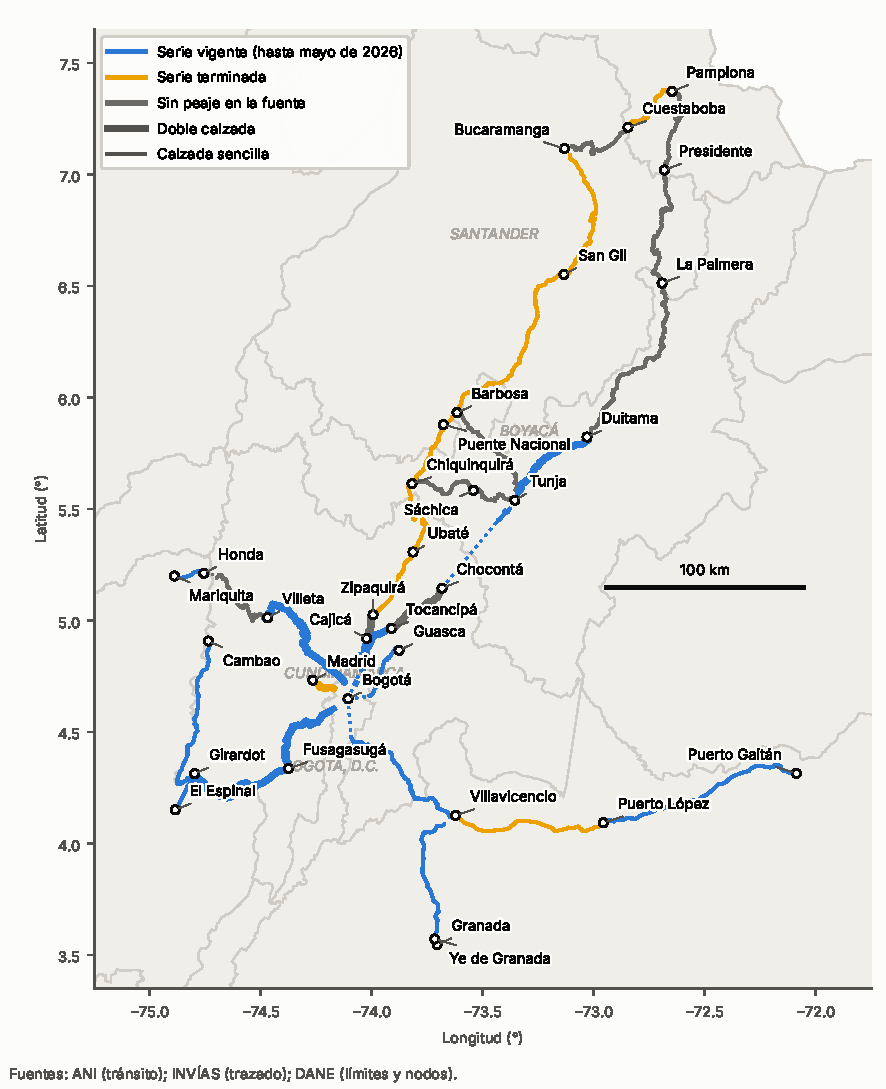
\includegraphics[width=0.86\textwidth]{c3_mapa_cobertura.pdf}
    \caption{Cobertura del dato de tránsito en la red. Fuente: elaboración propia}
    \label{fig:cobertura}
    \comoleerla{red de 32 tramos sobre el trazado de INVÍAS; el color es el estado de la serie de tránsito y el grosor, el tipo de calzada.}
{14 tramos tienen serie vigente, 7 serie terminada y 11 no tienen dato; 8 son de doble calzada.}
{el desvío por Santander no tiene ningún tramo con serie vigente: su tiempo estimado es, en su mayor parte, el tiempo libre.}

\end{figure}

\begin{figure}[H]
    \centering
    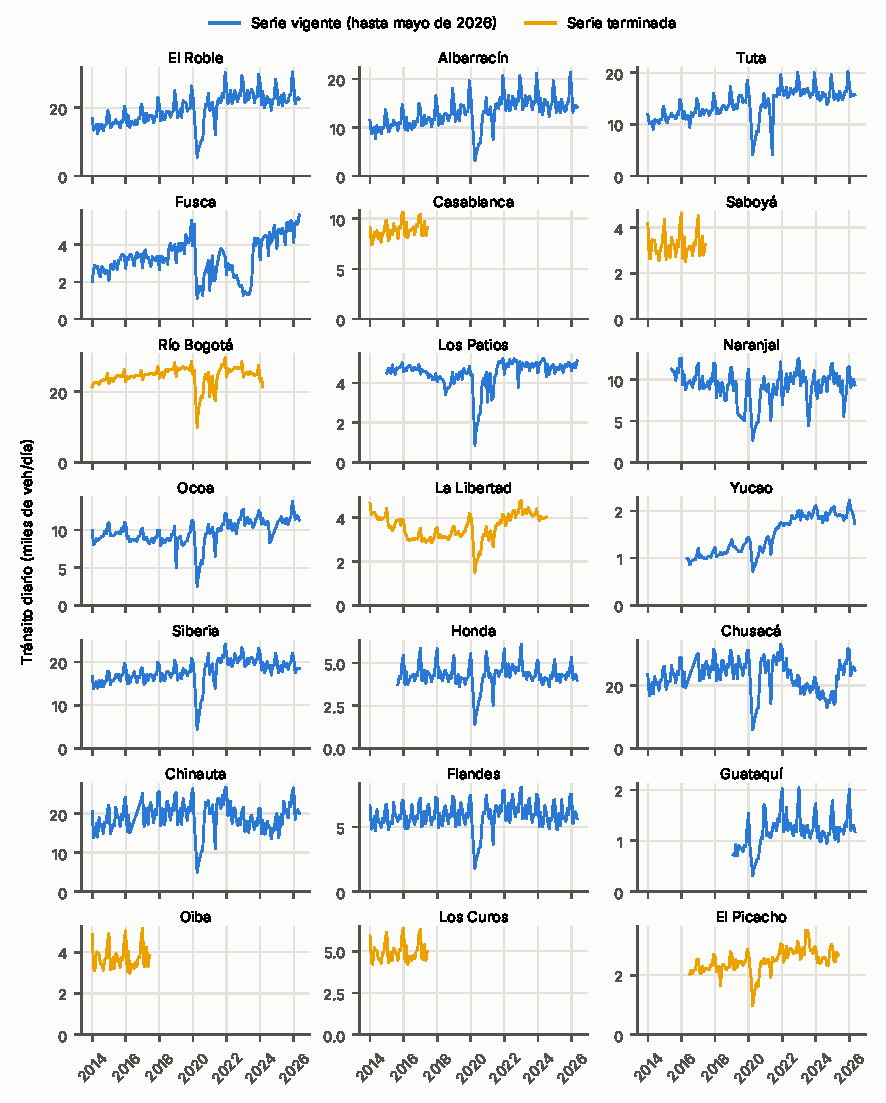
\includegraphics[width=\textwidth]{c3_series_red.pdf}
    \caption{Tránsito diario mensual de los peajes de la red. Fuente: elaboración propia}
    \label{fig:seriesred}
    \comoleerla{una gráfica por cada uno de los 21 peajes de la red que están en la fuente; el color indica si la serie llega al último mes.}
{14 series llegan a mayo de 2026 y 7 terminan antes; todas muestran la caída de 2020.}
{solo las series vigentes permiten pronosticar; en las terminadas el agente usa el mismo mes de su último año y lo rotula como histórico.}

\end{figure}

\section{Análisis exploratorio}
\label{sec:exploratorio}

El análisis usa las \ctFilasDepuradas{} filas depuradas. El tránsito diario
tiene una mediana de \ctTransitoMediano{} vehículos y un máximo de
\ctTransitoMaximo.

\begin{figure}[H]
    \centering
    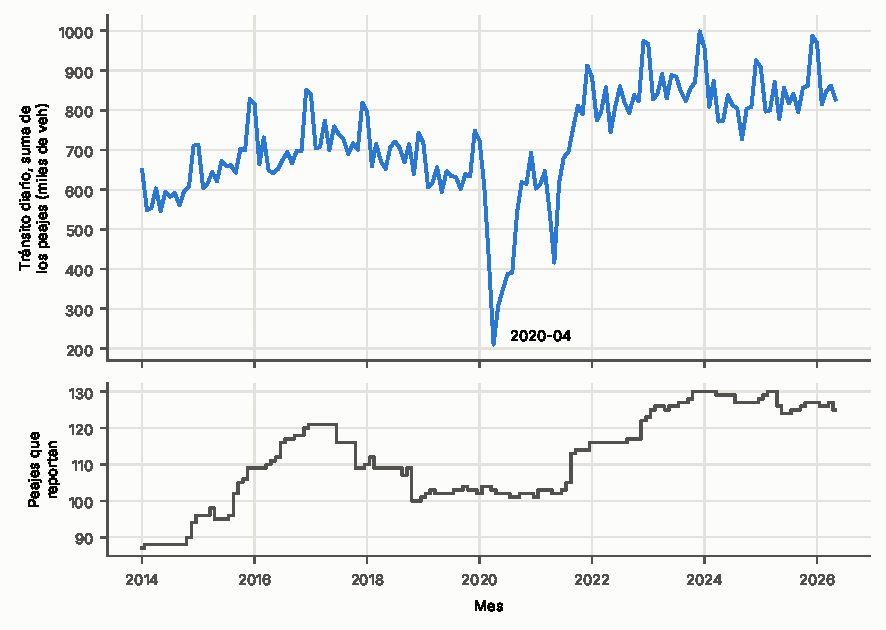
\includegraphics[width=0.95\textwidth]{c3_serie.pdf}
    \caption{Tránsito diario total y peajes que reportan, por mes. Fuente: elaboración propia}
    \label{fig:serie}
    \comoleerla{arriba, la suma del tránsito diario de todos los peajes que reportan en cada mes; abajo, cuántos peajes reportan.}
{el mínimo está en abril de 2020, un 68\,\% por debajo del mismo mes del año anterior; el número de peajes cambia con los años.}
{la suma mezcla el tránsito con la entrada y la salida de peajes de la fuente, por eso los modelos trabajan por peaje y no con el total.}

\end{figure}

\begin{figure}[H]
    \centering
    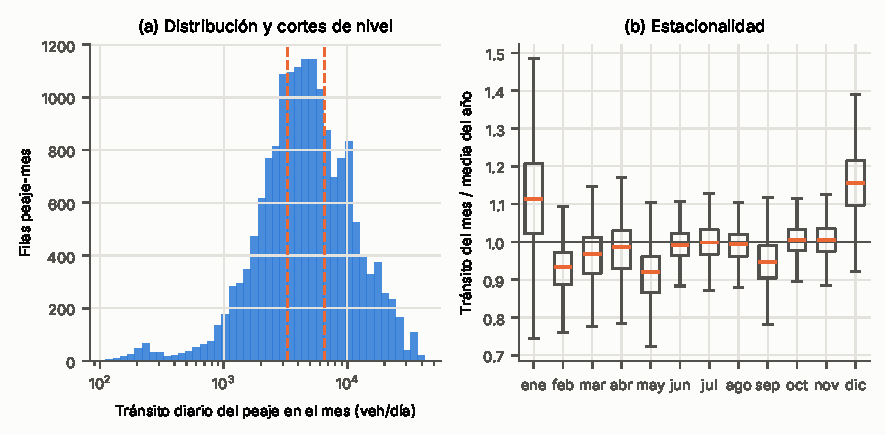
\includegraphics[width=\textwidth]{c3_distribucion.pdf}
    \caption{Distribución del tránsito diario y estacionalidad. Fuente: elaboración propia}
    \label{fig:distribucion}
    \comoleerla{(a) histograma del tránsito diario de las 16\,665 filas peaje-mes, en escala logarítmica, con los dos cortes de nivel; (b) tránsito de cada mes dividido por la media de su año, por mes calendario.}
{los cortes están en 3\,284 y 6\,564 vehículos por día; diciembre y enero quedan por encima de 1 y febrero y mayo por debajo.}
{los cortes son los terciles del entrenamiento; la estacionalidad justifica usar el mes del año y el rezago de 12 meses como predictores.}

\end{figure}

\begin{figure}[H]
    \centering
    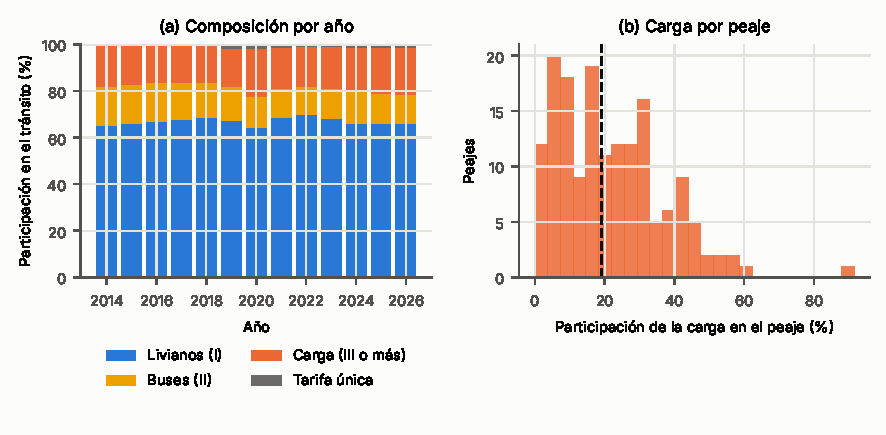
\includegraphics[width=\textwidth]{c3_composicion.pdf}
    \caption{Composición vehicular por año y por peaje. Fuente: elaboración propia}
    \label{fig:composicion}
    \comoleerla{(a) participación de cada grupo vehicular en el tránsito de cada año; (b) histograma de la participación de la carga por peaje.}
{en todo el periodo los livianos son el 67.2\,\%, los buses el 14.1\,\% y la carga el 17.8\,\%; entre peajes la carga varía mucho más que entre años.}
{la composición distingue corredores y por eso entra al agrupamiento; como cambia poco de un mes a otro, pesa poco en la regresión.}

\end{figure}

\begin{figure}[H]
    \centering
    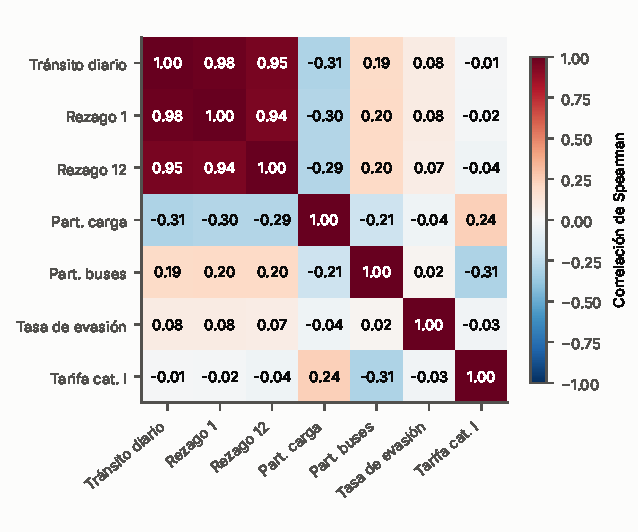
\includegraphics[width=0.74\textwidth]{c3_correlacion.pdf}
    \caption{Correlación entre las variables del conjunto modelable. Fuente: elaboración propia}
    \label{fig:correlacion}
    \comoleerla{correlación de Spearman entre las variables de las filas modelables; el tránsito y sus rezagos van en logaritmo.}
{el tránsito del mes se parece mucho al del mes anterior y al de 12 meses antes; la participación de la carga se relaciona de forma negativa con el tránsito.}
{esa persistencia explica que las referencias sin aprendizaje ya sean buenas y que el modelo deba medirse contra ellas.}

\end{figure}

\textbf{Lo que el análisis decide para los modelos.}
\begin{itemize}
\item El tránsito varía más de dos órdenes de magnitud entre peajes. El
objetivo de la regresión es su logaritmo.
\item El tránsito es persistente y estacional. Los predictores son rezagos
recientes, rezagos de un año y el mes.
\item La caída de \ctMesMinimo{} se conserva en los datos: es tránsito real.
Solo se excluye 2020 del perfil del agrupamiento, porque deforma la
estacionalidad.
\end{itemize}

\section{Diseño de los modelos}
\label{sec:diseno}

Los modelos están en \texttt{src/aprendizaje.py} y se ejecutan con
\texttt{experimentos/experimentos\_corte3.py}. Se usó
scikit-learn~\cite{sklearn} con la semilla 42.

\begin{itemize}
\item \textbf{Unidad de análisis:} un peaje en un mes.
\item \textbf{Pregunta:} con lo que se conoce al cierre de un mes, cuál será
el tránsito del mes siguiente.
\item \textbf{Predictores:} 19 columnas. Cinco rezagos en logaritmo, la
participación de la carga del mes anterior, los días del mes y doce
indicadores del mes del año.
\item \textbf{Partición:} temporal y sin barajar (Tabla~\ref{tab:particion}).
Barajar pondría meses futuros en el entrenamiento.
\item \textbf{Selección:} cada modelo se ajusta con el entrenamiento para
cada combinación de hiperparámetros y se elige la mejor en la validación.
Después se ajusta con entrenamiento más validación y se evalúa una sola vez
en la prueba.
\item \textbf{Referencias sin aprendizaje:} la persistencia (el valor del mes
anterior) y la estacional (el valor del mismo mes del año anterior). Un
modelo solo aporta si las supera.
\end{itemize}

\begin{table}[H]
\centering
\caption{Partición temporal de las filas modelables}
\label{tab:particion}
\small
\renewcommand{\arraystretch}{1.2}
\begin{tabular}{|l|l|r|r|}
\hline
\rowcolor{gray!20} \textbf{Conjunto} & \textbf{Periodo} & \textbf{Filas} & \textbf{Peajes} \\
\hline
\textbf{Entrenamiento} & 2015-02 a 2024-05 & 11\,348 & 151 \\
\hline
\textbf{Validación} & 2024-06 a 2025-05 & 1\,486 & 129 \\
\hline
\textbf{Prueba} & 2025-06 a 2026-05 & 1\,463 & 125 \\
\hline
\end{tabular}

\end{table}

\section{Regresión}
\label{sec:regresion}

Se compararon cuatro modelos: regresión lineal, árbol de decisión, bosque
aleatorio y potenciación del gradiente. El objetivo es el logaritmo del
tránsito diario; las métricas se calculan sobre el tránsito, en vehículos por
día.

\begin{table}[H]
\centering
\caption{Regresión del tránsito diario: referencias y modelos}
\label{tab:regresion}
\small\setlength{\tabcolsep}{4pt}
\renewcommand{\arraystretch}{1.2}
\begin{tabular}{|>{\raggedright\arraybackslash}p{4.6cm}|r|r|r|r|r|}
\hline
\rowcolor{gray!20} \textbf{Método} & \textbf{MAE val.} & \textbf{MAE} & \textbf{RMSE} & \textbf{$R^2$} & \textbf{EPM (\%)} \\
\hline
\textbf{Persistencia (mes anterior)} & 579.6 & 554.4 & 994.5 & 0.9735 & 5.97 \\
\hline
\textbf{Estacional (mismo mes del año anterior)} & 526.9 & 605.6 & 1\,297.3 & 0.9550 & 6.29 \\
\hline
\textbf{Regresión lineal} & 433.9 & 419.9 & 722.3 & 0.9860 & 4.78 \\
\hline
\textbf{Árbol de decisión} & 496.0 & 476.5 & 859.3 & 0.9803 & 5.57 \\
\hline
\textbf{Bosque aleatorio (elegido)} & 377.1 & 358.8 & 669.3 & 0.9880 & 3.94 \\
\hline
\textbf{Potenciación del gradiente} & 401.2 & 407.6 & 724.0 & 0.9860 & 4.67 \\
\hline
\end{tabular}

\comoleerla{una fila por método; MAE val. es el error absoluto medio en la validación, las demás columnas son de la prueba; EPM es el error porcentual mediano.}
{los cuatro modelos superan a las dos referencias en MAE en la prueba; el bosque aleatorio es el mejor en validación y en prueba, con $R^2 = 0.9880$.}
{el $R^2$ es alto incluso en las referencias porque el tránsito difiere mucho entre peajes; la comparación útil es el MAE.}

\end{table}

\begin{table}[H]
\centering
\caption{Hiperparámetros elegidos en la validación, regresión}
\label{tab:hiperreg}
\small
\renewcommand{\arraystretch}{1.2}
\begin{tabular}{|l|r|>{\raggedright\arraybackslash}p{7.2cm}|}
\hline
\rowcolor{gray!20} \textbf{Modelo} & \textbf{Combinaciones} & \textbf{Hiperparámetros elegidos} \\
\hline
\textbf{Regresión lineal} & 1 & sin hiperparámetros \\
\hline
\textbf{Árbol de decisión} & 10 & profundidad máxima 8, mínimo por hoja 20 \\
\hline
\textbf{Bosque aleatorio} & 6 & árboles 300, mínimo por hoja 1, variables 50\,\% por división \\
\hline
\textbf{Potenciación del gradiente} & 4 & tasa de aprendizaje 0.05, iteraciones 200 \\
\hline
\end{tabular}

\end{table}

\begin{figure}[H]
    \centering
    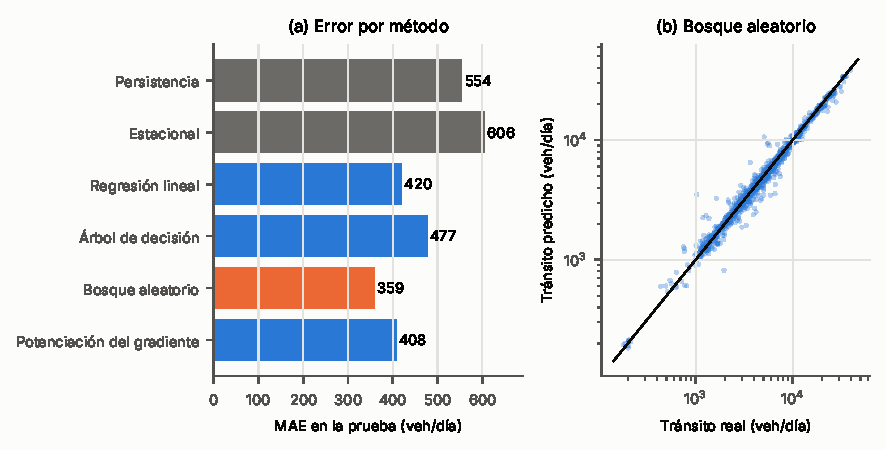
\includegraphics[width=\textwidth]{c3_regresion.pdf}
    \caption{Error por método y tránsito real contra predicho en la prueba. Fuente: elaboración propia}
    \label{fig:regresion}
    \comoleerla{(a) error absoluto medio en la prueba de las dos referencias (gris) y de los cuatro modelos; (b) tránsito real contra predicho del modelo elegido, en escala logarítmica.}
{el bosque aleatorio tiene el menor error, 358.8 vehículos por día, un 35\,\% menos que la persistencia (554.4); los puntos siguen la diagonal en todo el rango.}
{el modelo combina el nivel reciente con la estacionalidad, algo que ninguna de las dos referencias hace por separado.}

\end{figure}

\textbf{Resultado.}
\begin{itemize}
\item El \MakeLowercase{\ctMejorRegresor} tiene un MAE de \ctMaeMejor{}
vehículos por día y un error porcentual mediano de \ctEpmMejor\,\%.
\item La persistencia tiene \ctMaePersistencia{} y la estacional
\ctMaeEstacional. El modelo reduce el error un \ctMejoraMae\,\% frente a la
mejor referencia de la prueba.
\item La regresión lineal (\ctMaeLineal) queda por delante del árbol
(\ctMaeArbol): con rezagos en logaritmo, la relación es casi lineal.
\end{itemize}

\textbf{Pronóstico a varios meses.} Para los meses posteriores al último dato
no hay rezagos observados. El pronóstico es recursivo: cada mes predicho
entra como rezago del siguiente. Se midió lanzándolo al inicio de la prueba
y comparándolo con lo que pasó después (Figura~\ref{fig:horizonte}).

\begin{figure}[H]
    \centering
    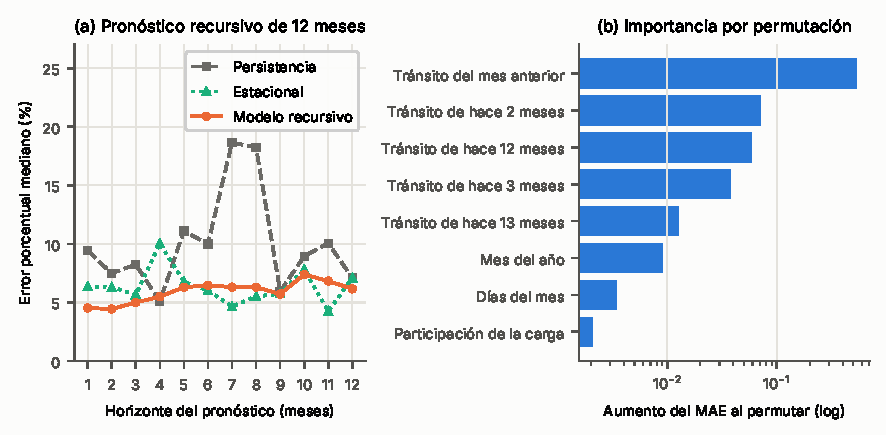
\includegraphics[width=\textwidth]{c3_horizonte.pdf}
    \caption{Error del pronóstico recursivo por horizonte e importancia de las variables. Fuente: elaboración propia}
    \label{fig:horizonte}
    \comoleerla{(a) error porcentual mediano del pronóstico recursivo lanzado al inicio de la prueba, por horizonte, frente a las dos referencias; (b) aumento del error al permutar cada variable.}
{el error del modelo pasa de 4.5\,\% a un mes a 6.2\,\% a doce; es el menor de los tres en 7 de los 12 horizontes. La variable que más pesa es el tránsito del mes anterior.}
{al encadenar predicciones el error se acumula, y a varios meses la referencia estacional alcanza al modelo; por eso el pronóstico de la red se rotula como tal.}

\end{figure}

\section{Clasificación}
\label{sec:clasificacion}

\textbf{Definición del nivel.} La fuente no mide congestión. El indicador del
proyecto es el nivel de tránsito diario del mes, en tres clases:
\begin{itemize}
\item \textbf{Bajo:} hasta \ctCorteBajo{} vehículos por día.
\item \textbf{Medio:} hasta \ctCorteAlto.
\item \textbf{Alto:} por encima de \ctCorteAlto.
\end{itemize}
Los cortes son los terciles del entrenamiento y quedan fijos. Mide la demanda
del tramo, no su saturación; la saturación se trata en la
Sección~\ref{sec:tiempo}.

Se compararon regresión logística, árbol de decisión y bosque aleatorio, con
los mismos predictores y la misma partición. La selección usa el F1 macro en
la validación.

\begin{table}[H]
\centering
\caption{Clasificación del nivel de tránsito: referencia y modelos}
\label{tab:clasificacion}
\small
\renewcommand{\arraystretch}{1.2}
\begin{tabular}{|>{\raggedright\arraybackslash}p{6.2cm}|r|r|r|}
\hline
\rowcolor{gray!20} \textbf{Método} & \textbf{F1 macro val. (\%)} & \textbf{Exactitud (\%)} & \textbf{F1 macro (\%)} \\
\hline
\textbf{Persistencia (clase del mes anterior)} & 91.96 & 91.39 & 91.47 \\
\hline
\textbf{Regresión logística} & 94.39 & 93.92 & 93.95 \\
\hline
\textbf{Árbol de decisión} & 94.72 & 93.30 & 93.39 \\
\hline
\textbf{Bosque aleatorio (elegido)} & 95.76 & 94.53 & 94.57 \\
\hline
\textbf{Clase a partir de la regresión} & no aplica & 94.19 & 94.26 \\
\hline
\end{tabular}

\end{table}

\begin{table}[H]
\centering
\caption{Hiperparámetros elegidos en la validación, clasificación}
\label{tab:hipercla}
\small
\renewcommand{\arraystretch}{1.2}
\begin{tabular}{|l|r|>{\raggedright\arraybackslash}p{7.2cm}|}
\hline
\rowcolor{gray!20} \textbf{Modelo} & \textbf{Combinaciones} & \textbf{Hiperparámetros elegidos} \\
\hline
\textbf{Regresión logística} & 3 & $C$ 10 \\
\hline
\textbf{Árbol de decisión} & 10 & profundidad máxima 8, mínimo por hoja 20 \\
\hline
\textbf{Bosque aleatorio} & 3 & árboles 300, mínimo por hoja 5 \\
\hline
\end{tabular}

\end{table}

\begin{figure}[H]
    \centering
    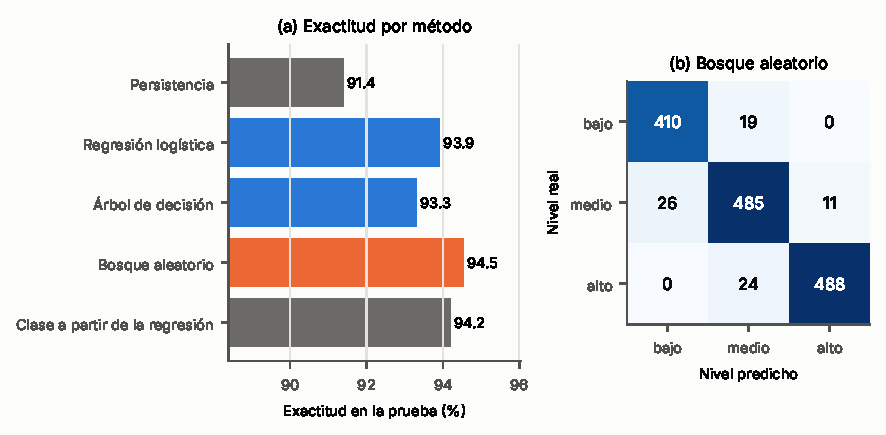
\includegraphics[width=\textwidth]{c3_clasificacion.pdf}
    \caption{Exactitud por método y matriz de confusión del clasificador elegido. Fuente: elaboración propia}
    \label{fig:clasificacion}
    \comoleerla{(a) exactitud en la prueba de la referencia, los tres clasificadores y la clase derivada de la regresión; (b) matriz de confusión del clasificador elegido.}
{el bosque aleatorio acierta el 94.53\,\% frente al 91.39\,\% de la persistencia; de sus 80 errores, 0 confunden bajo con alto.}
{los errores caen entre niveles vecinos, en peajes cuyo tránsito está cerca de un corte.}

\end{figure}

\begin{table}[H]
\centering
\caption{Métricas por nivel del clasificador elegido, en la prueba}
\label{tab:porclase}
\small
\renewcommand{\arraystretch}{1.2}
\begin{tabular}{|l|r|r|r|r|}
\hline
\rowcolor{gray!20} \textbf{Nivel} & \textbf{Precisión (\%)} & \textbf{Exhaustividad (\%)} & \textbf{F1 (\%)} & \textbf{Casos} \\
\hline
\textbf{Bajo} & 94.04 & 95.57 & 94.80 & 429 \\
\hline
\textbf{Medio} & 91.86 & 92.91 & 92.38 & 522 \\
\hline
\textbf{Alto} & 97.80 & 95.31 & 96.54 & 512 \\
\hline
\end{tabular}

\end{table}

\textbf{Resultado.}
\begin{itemize}
\item El \MakeLowercase{\ctMejorClasificador} acierta el
\ctExactitudMejor\,\% de los \ctFilasPrueba{} casos de la prueba, con F1
macro de \ctFunoMejor\,\%.
\item La persistencia acierta el \ctExactitudPersistencia\,\%. La ventaja del
modelo es de pocos puntos porque el nivel de un peaje cambia poco de un mes a
otro.
\item Convertir en clase la predicción de la regresión da
\ctExactitudDerivada\,\%, casi lo mismo. Los dos caminos son coherentes.
\item Ningún error confunde bajo con alto (\ctErroresExtremos{} casos).
\end{itemize}

\section{Agrupamiento}
\label{sec:agrupamiento}

\textbf{Perfil de cada peaje.} Entran los \ctPeajesAgrupados{} peajes con al
menos 24 meses depurados y dos años calendario completos. Cada uno se
describe con cuatro variables estandarizadas:
\begin{itemize}
\item logaritmo del tránsito diario medio;
\item participación de la carga;
\item participación de los buses;
\item amplitud estacional: diferencia entre el mes más alto y el más bajo,
cada uno relativo a la media de su año.
\end{itemize}
Se calcularon dos variables más, el índice de diciembre y enero y el
crecimiento anual, y no entraron: la primera repite la amplitud estacional y
la segunda la dominan las series cortas.

\textbf{Métodos.} K-medias y agrupamiento jerárquico con enlace de Ward. El
número de grupos es el de mayor silueta de K-medias entre 2 y 8.

\begin{figure}[H]
    \centering
    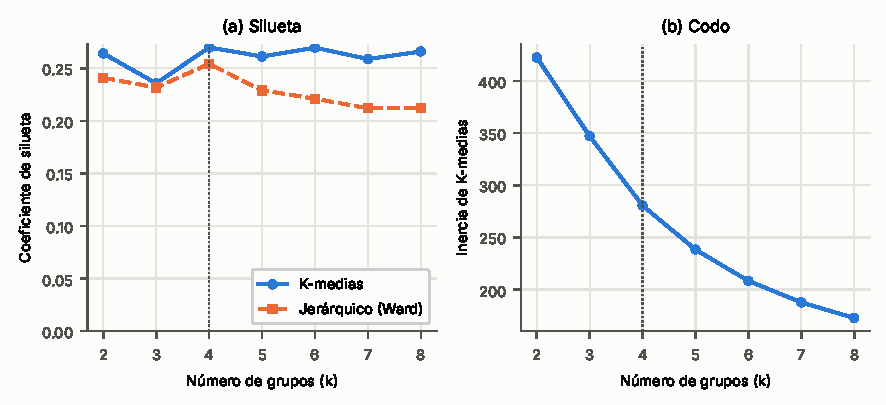
\includegraphics[width=0.95\textwidth]{c3_silueta.pdf}
    \caption{Silueta e inercia según el número de grupos. Fuente: elaboración propia}
    \label{fig:silueta}
    \comoleerla{(a) coeficiente de silueta de K-medias y del jerárquico para cada número de grupos; (b) inercia de K-medias.}
{la mayor silueta de K-medias está en k = 4 (0.270); la curva es casi plana y la inercia no tiene un codo marcado.}
{una silueta cercana a 0.27 indica grupos que se tocan: los peajes forman un continuo y los grupos son una división útil, no clases separadas.}

\end{figure}

\begin{figure}[H]
    \centering
    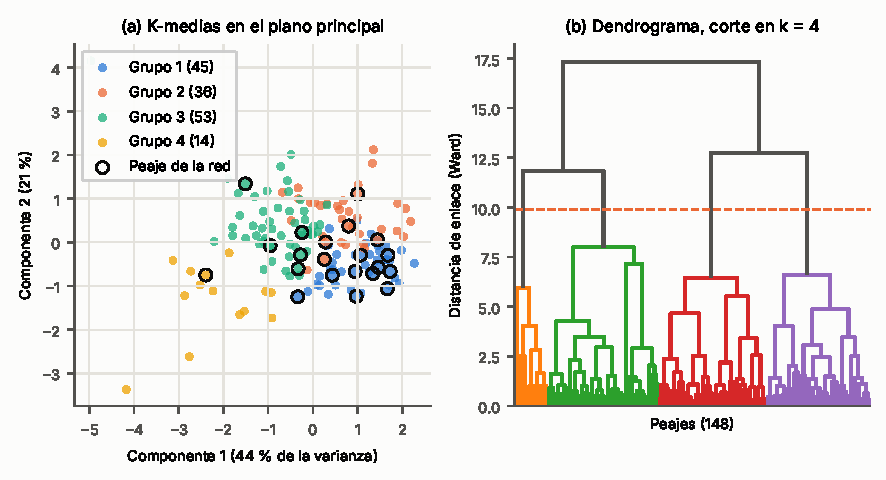
\includegraphics[width=\textwidth]{c3_grupos.pdf}
    \caption{Grupos de K-medias en el plano principal y dendrograma de Ward. Fuente: elaboración propia}
    \label{fig:grupos}
    \comoleerla{(a) los 148 peajes en el plano de las dos componentes principales, con el grupo de K-medias; el borde negro marca los peajes de la red; (b) dendrograma del agrupamiento jerárquico con el corte.}
{el plano recoge el 65\,\% de la varianza; los dos métodos coinciden con un índice de Rand ajustado de 0.77.}
{que dos métodos distintos lleguen a grupos parecidos respalda la división, aunque la silueta sea baja.}

\end{figure}

\begin{table}[H]
\centering
\caption{Perfil medio de los grupos de K-medias}
\label{tab:grupos}
\small
\renewcommand{\arraystretch}{1.2}
\begin{tabular}{|l|r|r|r|r|r|}
\hline
\rowcolor{gray!20} \textbf{Grupo} & \textbf{Peajes} & \textbf{Tránsito (veh/día)} & \textbf{Carga (\%)} & \textbf{Buses (\%)} & \textbf{Amplitud} \\
\hline
\textbf{Grupo 1} & 45 & 11\,087 & 8.9 & 12.3 & 0.26 \\
\hline
\textbf{Grupo 2} & 36 & 5\,283 & 20.3 & 27.6 & 0.31 \\
\hline
\textbf{Grupo 3} & 53 & 3\,869 & 34.0 & 8.0 & 0.30 \\
\hline
\textbf{Grupo 4} & 14 & 1\,704 & 22.8 & 4.6 & 0.71 \\
\hline
\end{tabular}

\end{table}

\begin{table}[H]
\centering
\caption{Peajes de la red en cada grupo}
\label{tab:gruposred}
\small
\renewcommand{\arraystretch}{1.2}
\begin{tabular}{|l|r|>{\raggedright\arraybackslash}p{9.4cm}|}
\hline
\rowcolor{gray!20} \textbf{Grupo} & \textbf{En la red} & \textbf{Peajes de la red} \\
\hline
\textbf{Grupo 1} & 10 & Chinauta, Chusaca, Río Bogotá, Los Patios, Siberia, Fusca, El Roble, Albarracín, Ocoa, Tuta \\
\hline
\textbf{Grupo 2} & 5 & El Picacho, Los Curos, Oiba, Saboyá, Casablanca \\
\hline
\textbf{Grupo 3} & 5 & Honda, Naranjal, Flandes, La Libertad, Yucao \\
\hline
\textbf{Grupo 4} & 1 & Guataquí \\
\hline
\end{tabular}

\end{table}

\textbf{Resultado.}
\begin{itemize}
\item Con $k = \ctKGrupos$ la silueta es \ctSiluetaKmedias{} en K-medias y
\ctSiluetaJerarquico{} en el jerárquico. Son valores bajos: los peajes forman
un continuo.
\item Los dos métodos coinciden con un índice de Rand ajustado de
\ctRandAjustado.
\item El grupo \ctGrupoMayor{} reúne los corredores de mayor tránsito
(\ctGrupoMayorTransito{} vehículos por día en promedio) y contiene
\ctGrupoMayorEnRed{} peajes de la red, los de los accesos a Bogotá.
\item El grupo \ctGrupoEstacional{} es el más estacional (amplitud
\ctGrupoEstacionalAmplitud) y el de menor tránsito.
\end{itemize}

\section{Tiempo de recorrido}
\label{sec:tiempo}

El tiempo de un tramo se estima con la función BPR~\cite{bpr}:
\[
t = t_{\text{libre}}\left(1 + \alpha\left(\frac{v}{c}\right)^{\beta}\right),
\qquad t_{\text{libre}} = \frac{d}{v_{\text{libre}}},
\qquad v = K \cdot \text{tránsito diario}
\]
donde $d$ es la distancia del tramo, $c$ la capacidad de la calzada y $K$ el
factor de hora pico. Está en \texttt{src/modelo\_tiempo.py} y sus insumos en
\texttt{config\_tiempo.json} (Tabla~\ref{tab:supuestos}).

\begin{table}[H]
\centering
\caption{Insumos del tiempo estimado y su estado}
\label{tab:supuestos}
\small
\renewcommand{\arraystretch}{1.2}
\begin{tabular}{|l|r|l|}
\hline
\rowcolor{gray!20} \textbf{Insumo} & \textbf{Valor} & \textbf{Estado} \\
\hline
\textbf{Velocidad libre} & 50 km/h & supuesto del equipo \\
\hline
\textbf{$\alpha$ de la función BPR} & 0.15 & supuesto del equipo \\
\hline
\textbf{$\beta$ de la función BPR} & 4 & supuesto del equipo \\
\hline
\textbf{Factor de hora pico} & 0.10 & supuesto del equipo \\
\hline
\textbf{Capacidad, calzada sencilla} & 3\,200 veh/h & supuesto del equipo \\
\hline
\textbf{Capacidad, doble calzada} & 8\,800 veh/h & supuesto del equipo \\
\hline
\textbf{Banda de doble calzada} & 1.7 a 2.3 & verificada \\
\hline
\end{tabular}

\end{table}

\textbf{Qué es dato y qué es supuesto.}
\begin{itemize}
\item \textbf{Datos:} la distancia (INVÍAS, con el piso geodésico del
Corte 2), el tránsito (ANI) y el tipo de calzada. La doble calzada sale de
los datos del proyecto: INVÍAS digitaliza las dos calzadas y la razón entre
la longitud digitalizada y la registrada queda en la banda que el Corte 1
verificó. Hay \ctTramosDobleCalzada{} tramos de doble calzada.
\item \textbf{Supuestos:} la velocidad libre de \ctVelocidadLibre{} km/h (la
misma del visualizador del Corte 2), $\alpha$, $\beta$, el factor de hora
pico y las dos capacidades.
\end{itemize}

\begin{figure}[H]
    \centering
    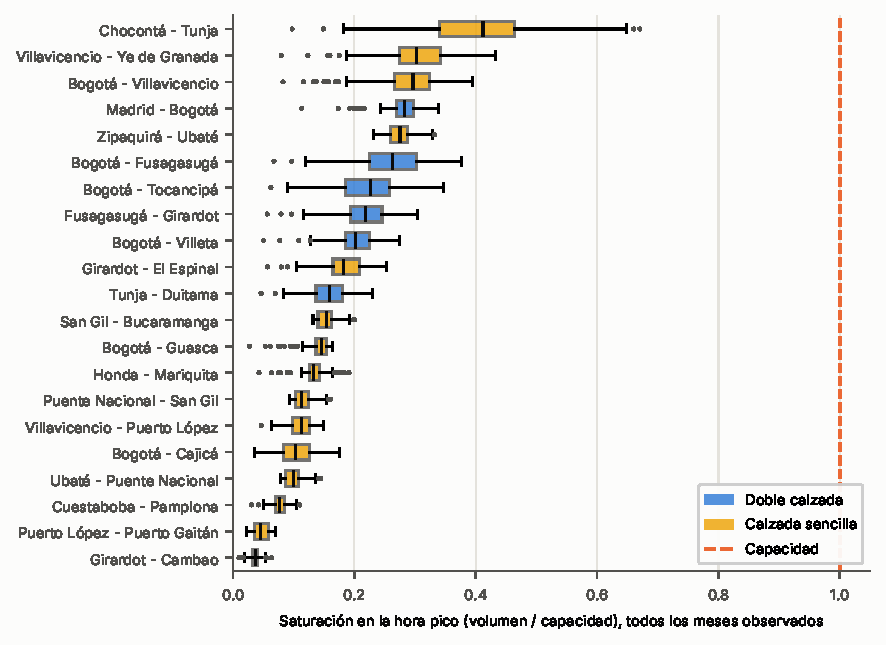
\includegraphics[width=0.95\textwidth]{c3_saturacion.pdf}
    \caption{Saturación en la hora pico de los tramos de la red. Fuente: elaboración propia}
    \label{fig:saturacion}
    \comoleerla{saturación en la hora pico de cada tramo de la red con peaje en la fuente, en todos sus meses observados (2\,450 filas); la línea punteada es la capacidad.}
{la mediana es 0.18 y el máximo 0.67, en Chocontá - Tunja; ningún tramo llega a la capacidad.}
{con promedios mensuales el volumen queda lejos de la capacidad y el término de congestión de la función BPR casi no pesa.}

\end{figure}

\begin{table}[H]
\centering
\caption{Saturación, demora y error del tiempo estimado}
\label{tab:tiempo}
\small
\renewcommand{\arraystretch}{1.2}
\begin{tabular}{|l|r|}
\hline
\rowcolor{gray!20} \textbf{Medida} & \textbf{Valor} \\
\hline
\textbf{Filas tramo-mes con tránsito observado} & 2\,450 \\
\hline
\textbf{Saturación mediana} & 0.18 \\
\hline
\textbf{Saturación máxima} & 0.67 \\
\hline
\textbf{Factor BPR máximo} & 1.0303 \\
\hline
\textbf{Mayor demora de un tramo en un mes (min)} & 2.07 \\
\hline
\textbf{Casos tramo-mes en la prueba} & 162 \\
\hline
\textbf{Error absoluto medio del tiempo en la prueba (min)} & 0.019 \\
\hline
\textbf{Error máximo del tiempo en la prueba (min)} & 0.74 \\
\hline
\end{tabular}

\end{table}

\textbf{Resultado.}
\begin{itemize}
\item La mayor demora de un tramo en un mes es de \ctDemoraMaxima{} minutos,
en \ctTramoDemoraMaxima{} en \ctMesDemoraMaxima.
\item En los \ctCasosTiempo{} casos tramo-mes de la prueba, el tiempo
calculado con el tránsito predicho difiere del calculado con el tránsito
observado en \ctMaeTiempo{} minutos en promedio y \ctErrorMaximoTiempo{} como
máximo.
\item El error es pequeño porque el tiempo depende poco del tránsito en este
rango de saturación, no porque la predicción del tiempo sea difícil de
fallar. Con promedios mensuales, el tiempo estimado es casi el tiempo libre.
\end{itemize}

\section{Integración}
\label{sec:integracion}

\subsection{Agente predictivo}

El agente está en \texttt{src/agente\_predictivo.py}. No entrena ni carga
modelos: lee \nolinkurl{outputs/datos/pronostico_red.json}, que el
experimento escribe con el tránsito, el nivel y el tiempo de cada tramo para
24 meses (los 12 de la prueba y los 12 siguientes al último dato).

\textbf{Funcionamiento.}
\begin{enumerate}
\item \textbf{Percepción.} Recibe origen, destino y mes. Pone en cada arista
del grafo el tiempo estimado, el nivel de tránsito y el origen del dato.
\item \textbf{Búsqueda.} Ejecuta el A* del Corte 2
(\texttt{src/busquedas.py}) con el tiempo como costo.
\item \textbf{Comparación.} Evalúa las demás rutas simples entre el origen y
el destino. La red tiene un solo ciclo, de modo que hay una o dos.
\item \textbf{Avisos.} Informa los tramos con tránsito alto, los tramos sin
dato y los que usan una serie terminada.
\end{enumerate}

\textbf{Origen del dato de cada tramo.}
\begin{itemize}
\item \textbf{Predicción a un mes:} meses de la prueba, con rezagos
observados.
\item \textbf{Pronóstico recursivo:} meses posteriores a \ctUltimoMes, con el
modelo reajustado con todos los datos y los mismos hiperparámetros.
\item \textbf{Histórico:} series terminadas; se usa el mismo mes de su último
año.
\item \textbf{Sin dato:} el tramo usa el tiempo libre.
\end{itemize}

\textbf{Heurística.} Para el criterio de tiempo,
$h(n) = 60\, d_{\text{geo}}(n, \text{meta}) / v_{\text{libre}}$, en minutos.
\begin{itemize}
\item El tiempo de un tramo no es menor que su tiempo libre, porque el factor
de la BPR es mayor o igual que 1.
\item La distancia de un tramo no es menor que la geodésica entre sus nodos,
por el piso geodésico del Corte 2.
\item Por tanto $h(u) \le t(u, v) + h(v)$ en toda arista: $h$ es consistente
y admisible, y A* no reexpande nodos.
\end{itemize}
Las pruebas lo comprueban en los 24 meses, y comparan A* con Dijkstra en los
992 pares ordenados de dos meses.

\subsection{Caso central}

En \ctMesEjemplo, de Duitama a Puente Nacional, A* expande
\ctCasoExpandidos{} nodos y devuelve la ruta por Bogotá
(Figura~\ref{fig:mapanivel}, Tabla~\ref{tab:caso}).

\begin{figure}[H]
    \centering
    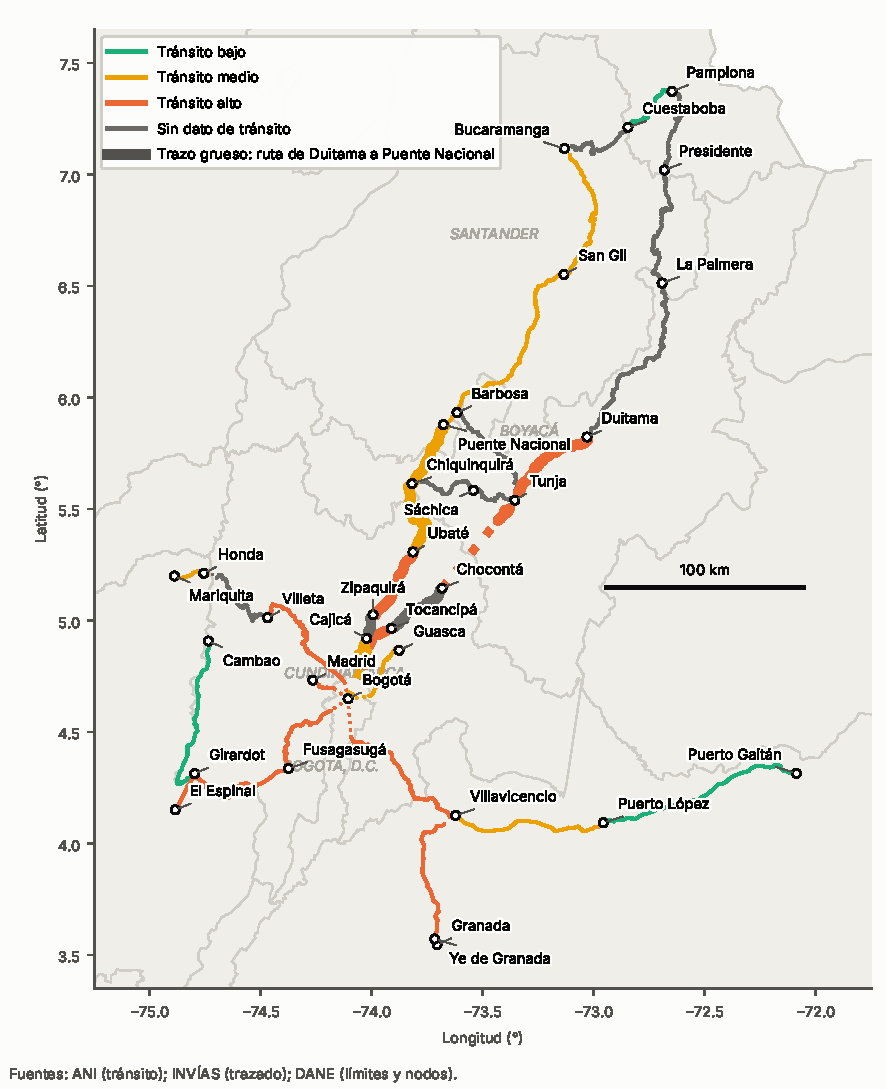
\includegraphics[width=0.86\textwidth]{c3_mapa_nivel.pdf}
    \caption{Nivel de tránsito previsto y ruta recomendada en el caso central. Fuente: elaboración propia}
    \label{fig:mapanivel}
    \comoleerla{nivel de tránsito previsto de cada tramo en diciembre de 2026 y, en trazo grueso, la ruta de menor tiempo estimado de Duitama a Puente Nacional.}
{la ruta mide 370.54 km y tarda 7 h 27 min; 4 de sus 8 tramos tienen tránsito alto y 2 no tienen dato.}
{la alternativa evita los tramos en alto pero tarda 339 minutos más: la distancia decide la ruta y el nivel de tránsito informa del estado esperado del recorrido.}

\end{figure}

\begin{table}[H]
\centering
\caption{Ruta recomendada y alternativa en el caso central}
\label{tab:caso}
\small
\renewcommand{\arraystretch}{1.2}
\begin{tabular}{|l|r|r|r|r|r|}
\hline
\rowcolor{gray!20} \textbf{Ruta} & \textbf{km} & \textbf{Tiempo} & \textbf{Demora (min)} & \textbf{En alto} & \textbf{Sin dato} \\
\hline
\textbf{Recomendada (por Bogotá)} & 370.54 & 7 h 27 min & 1.84 & 4 & 2 \\
\hline
\textbf{Alternativa (por Santander)} & 654.25 & 13 h 05 min & 0.03 & 0 & 4 \\
\hline
\end{tabular}

\end{table}

\begin{table}[H]
\centering
\caption{El caso central en los 12 meses del pronóstico}
\label{tab:casomeses}
\small
\renewcommand{\arraystretch}{1.2}
\begin{tabular}{|l|r|r|r|r|r|}
\hline
\rowcolor{gray!20} \textbf{Mes} & \textbf{Tiempo (min)} & \textbf{Demora (min)} & \textbf{Alto} & \textbf{Medio} & \textbf{Bajo} \\
\hline
\textbf{Junio de 2026} & 445.4 & 0.76 & 4 & 1 & 1 \\
\hline
\textbf{Julio de 2026} & 445.2 & 0.60 & 4 & 1 & 1 \\
\hline
\textbf{Agosto de 2026} & 445.2 & 0.56 & 4 & 1 & 1 \\
\hline
\textbf{Septiembre de 2026} & 445.1 & 0.50 & 4 & 1 & 1 \\
\hline
\textbf{Octubre de 2026} & 445.3 & 0.65 & 4 & 2 & 0 \\
\hline
\textbf{Noviembre de 2026} & 445.3 & 0.63 & 4 & 1 & 1 \\
\hline
\textbf{Diciembre de 2026} & 446.5 & 1.84 & 4 & 2 & 0 \\
\hline
\textbf{Enero de 2027} & 445.8 & 1.15 & 4 & 2 & 0 \\
\hline
\textbf{Febrero de 2027} & 445.1 & 0.41 & 4 & 1 & 1 \\
\hline
\textbf{Marzo de 2027} & 445.2 & 0.51 & 4 & 1 & 1 \\
\hline
\textbf{Abril de 2027} & 445.3 & 0.67 & 4 & 2 & 0 \\
\hline
\textbf{Mayo de 2027} & 445.2 & 0.56 & 4 & 1 & 1 \\
\hline
\end{tabular}

\comoleerla{la ruta recomendada de Duitama a Puente Nacional en cada mes del pronóstico: tiempo, demora y número de tramos por nivel.}
{la demora va de 0.41 a 1.84 minutos; la ruta es la misma los 12 meses.}
{lo que cambia de un mes a otro es el nivel de algunos tramos, no la decisión.}

\end{table}

\begin{table}[H]
\centering
\caption{Tránsito y nivel previstos por tramo con peaje}
\label{tab:red}
\footnotesize\setlength{\tabcolsep}{3pt}
\renewcommand{\arraystretch}{1.2}
\begin{tabular}{|>{\raggedright\arraybackslash}p{3.5cm}|>{\raggedright\arraybackslash}p{2.0cm}|>{\raggedright\arraybackslash}p{2.5cm}|l|r|>{\raggedright\arraybackslash}p{2.1cm}|}
\hline
\rowcolor{gray!20} \textbf{Tramo} & \textbf{Peaje} & \textbf{Serie} & \textbf{Calzada} & \textbf{Veh/día} & \textbf{Nivel ($v/c$)} \\
\hline
\textbf{Bogotá - Tocancipá} & El Roble & vigente & doble & 28\,981 & alto (0.33) \\
\hline
\textbf{Chocontá - Tunja} & Albarracín & vigente & sencilla & 20\,199 & alto (0.63) \\
\hline
\textbf{Tunja - Duitama} & Tuta & vigente & doble & 19\,710 & alto (0.22) \\
\hline
\textbf{Barbosa - Tunja} & Arcabuco & sin dato & sencilla & sin dato & sin dato \\
\hline
\textbf{Sáchica - Tunja} & Sáchica & sin dato & sencilla & sin dato & sin dato \\
\hline
\textbf{Bogotá - Cajicá} & Fusca & vigente & sencilla & 5\,192 & medio (0.16) \\
\hline
\textbf{Zipaquirá - Ubaté} & Casablanca & terminada (2017-06) & sencilla & 10\,322 & alto (0.32) \\
\hline
\textbf{Ubaté - Puente Nacional} & Saboyá & terminada (2017-06) & sencilla & 3\,955 & medio (0.12) \\
\hline
\textbf{Madrid - Bogotá} & Río Bogotá & terminada (2024-03) & doble & 27\,566 & alto (0.31) \\
\hline
\textbf{Bogotá - Guasca} & Los Patios & vigente & sencilla & 4\,942 & medio (0.15) \\
\hline
\textbf{Bogotá - Villavicencio} & Naranjal & vigente & sencilla & 10\,741 & alto (0.34) \\
\hline
\textbf{Villavicencio - Ye de Granada} & Ocoa & vigente & sencilla & 13\,006 & alto (0.41) \\
\hline
\textbf{Villavicencio - Puerto López} & La Libertad & terminada (2024-07) & sencilla & 4\,405 & medio (0.14) \\
\hline
\textbf{Puerto López - Puerto Gaitán} & Yucao & vigente & sencilla & 2\,126 & bajo (0.07) \\
\hline
\textbf{Bogotá - Villeta} & Siberia & vigente & doble & 22\,109 & alto (0.25) \\
\hline
\textbf{Villeta - Honda} & Bicentenario & sin dato & sencilla & sin dato & sin dato \\
\hline
\textbf{Honda - Mariquita} & Honda & vigente & sencilla & 4\,707 & medio (0.15) \\
\hline
\textbf{Bogotá - Fusagasugá} & Chusacá & vigente & doble & 29\,016 & alto (0.33) \\
\hline
\textbf{Fusagasugá - Girardot} & Chinauta & vigente & doble & 24\,284 & alto (0.28) \\
\hline
\textbf{Girardot - El Espinal} & Flandes & vigente & sencilla & 7\,206 & alto (0.23) \\
\hline
\textbf{Girardot - Cambao} & Guataquí & vigente & sencilla & 1\,468 & bajo (0.05) \\
\hline
\textbf{Puente Nacional - San Gil} & Oiba & terminada (2017-06) & sencilla & 4\,690 & medio (0.15) \\
\hline
\textbf{San Gil - Bucaramanga} & Los Curos & terminada (2017-06) & sencilla & 6\,038 & medio (0.19) \\
\hline
\textbf{Cuestaboba - Pamplona} & El Picacho & terminada (2025-05) & sencilla & 3\,042 & bajo (0.10) \\
\hline
\end{tabular}

\end{table}

La Tabla~\ref{tab:red} corresponde a \ctMesEjemplo. La
Figura~\ref{fig:pronosticored} muestra el pronóstico de los
\ctTramosVigentes{} tramos con serie vigente.

\begin{figure}[H]
    \centering
    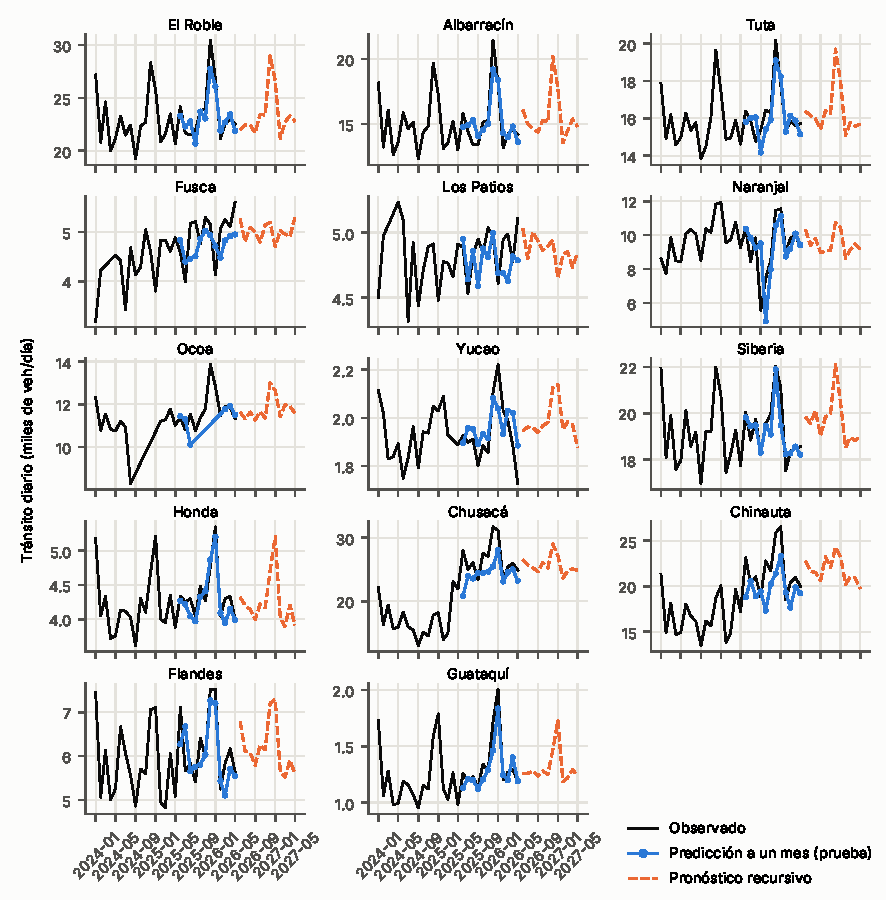
\includegraphics[width=\textwidth]{c3_pronostico_red.pdf}
    \caption{Tránsito observado, predicho y pronosticado en los peajes vigentes de la red. Fuente: elaboración propia}
    \label{fig:pronosticored}
    \comoleerla{los 14 peajes de la red con serie vigente desde 2024: observado, predicción a un mes en la prueba y pronóstico recursivo de los 12 meses siguientes.}
{la predicción a un mes sigue los picos de diciembre y enero; el pronóstico repite esa forma hacia adelante.}
{el pronóstico hereda la estacionalidad del rezago de 12 meses; no anticipa cierres ni cambios de operación como los que cortaron algunas series.}

\end{figure}

\subsection{Aplicación web}

El visualizador del Corte 2 (FastAPI y Leaflet) tiene una página nueva,
\texttt{/aprendizaje}, enlazada desde la cabecera
(Figura~\ref{fig:interfaz}).

\begin{itemize}
\item \textbf{Entrada:} mes, origen y destino.
\item \textbf{Mapa:} cada tramo con el color de su nivel de tránsito y la
ruta recomendada en trazo grueso.
\item \textbf{Ruta:} tiempo estimado, demora, distancia, detalle por tramo,
alternativa y avisos.
\item \textbf{Modelos:} cuatro pestañas con las métricas de la regresión, la
clasificación y el agrupamiento, y los supuestos del tiempo.
\item \textbf{Servidor:} tres rutas nuevas bajo
\texttt{/api/aprendizaje/}. El servidor lee los resultados guardados y no
importa scikit-learn, de modo que el despliegue no cambia de dependencias.
\end{itemize}

\begin{figure}[H]
    \centering
    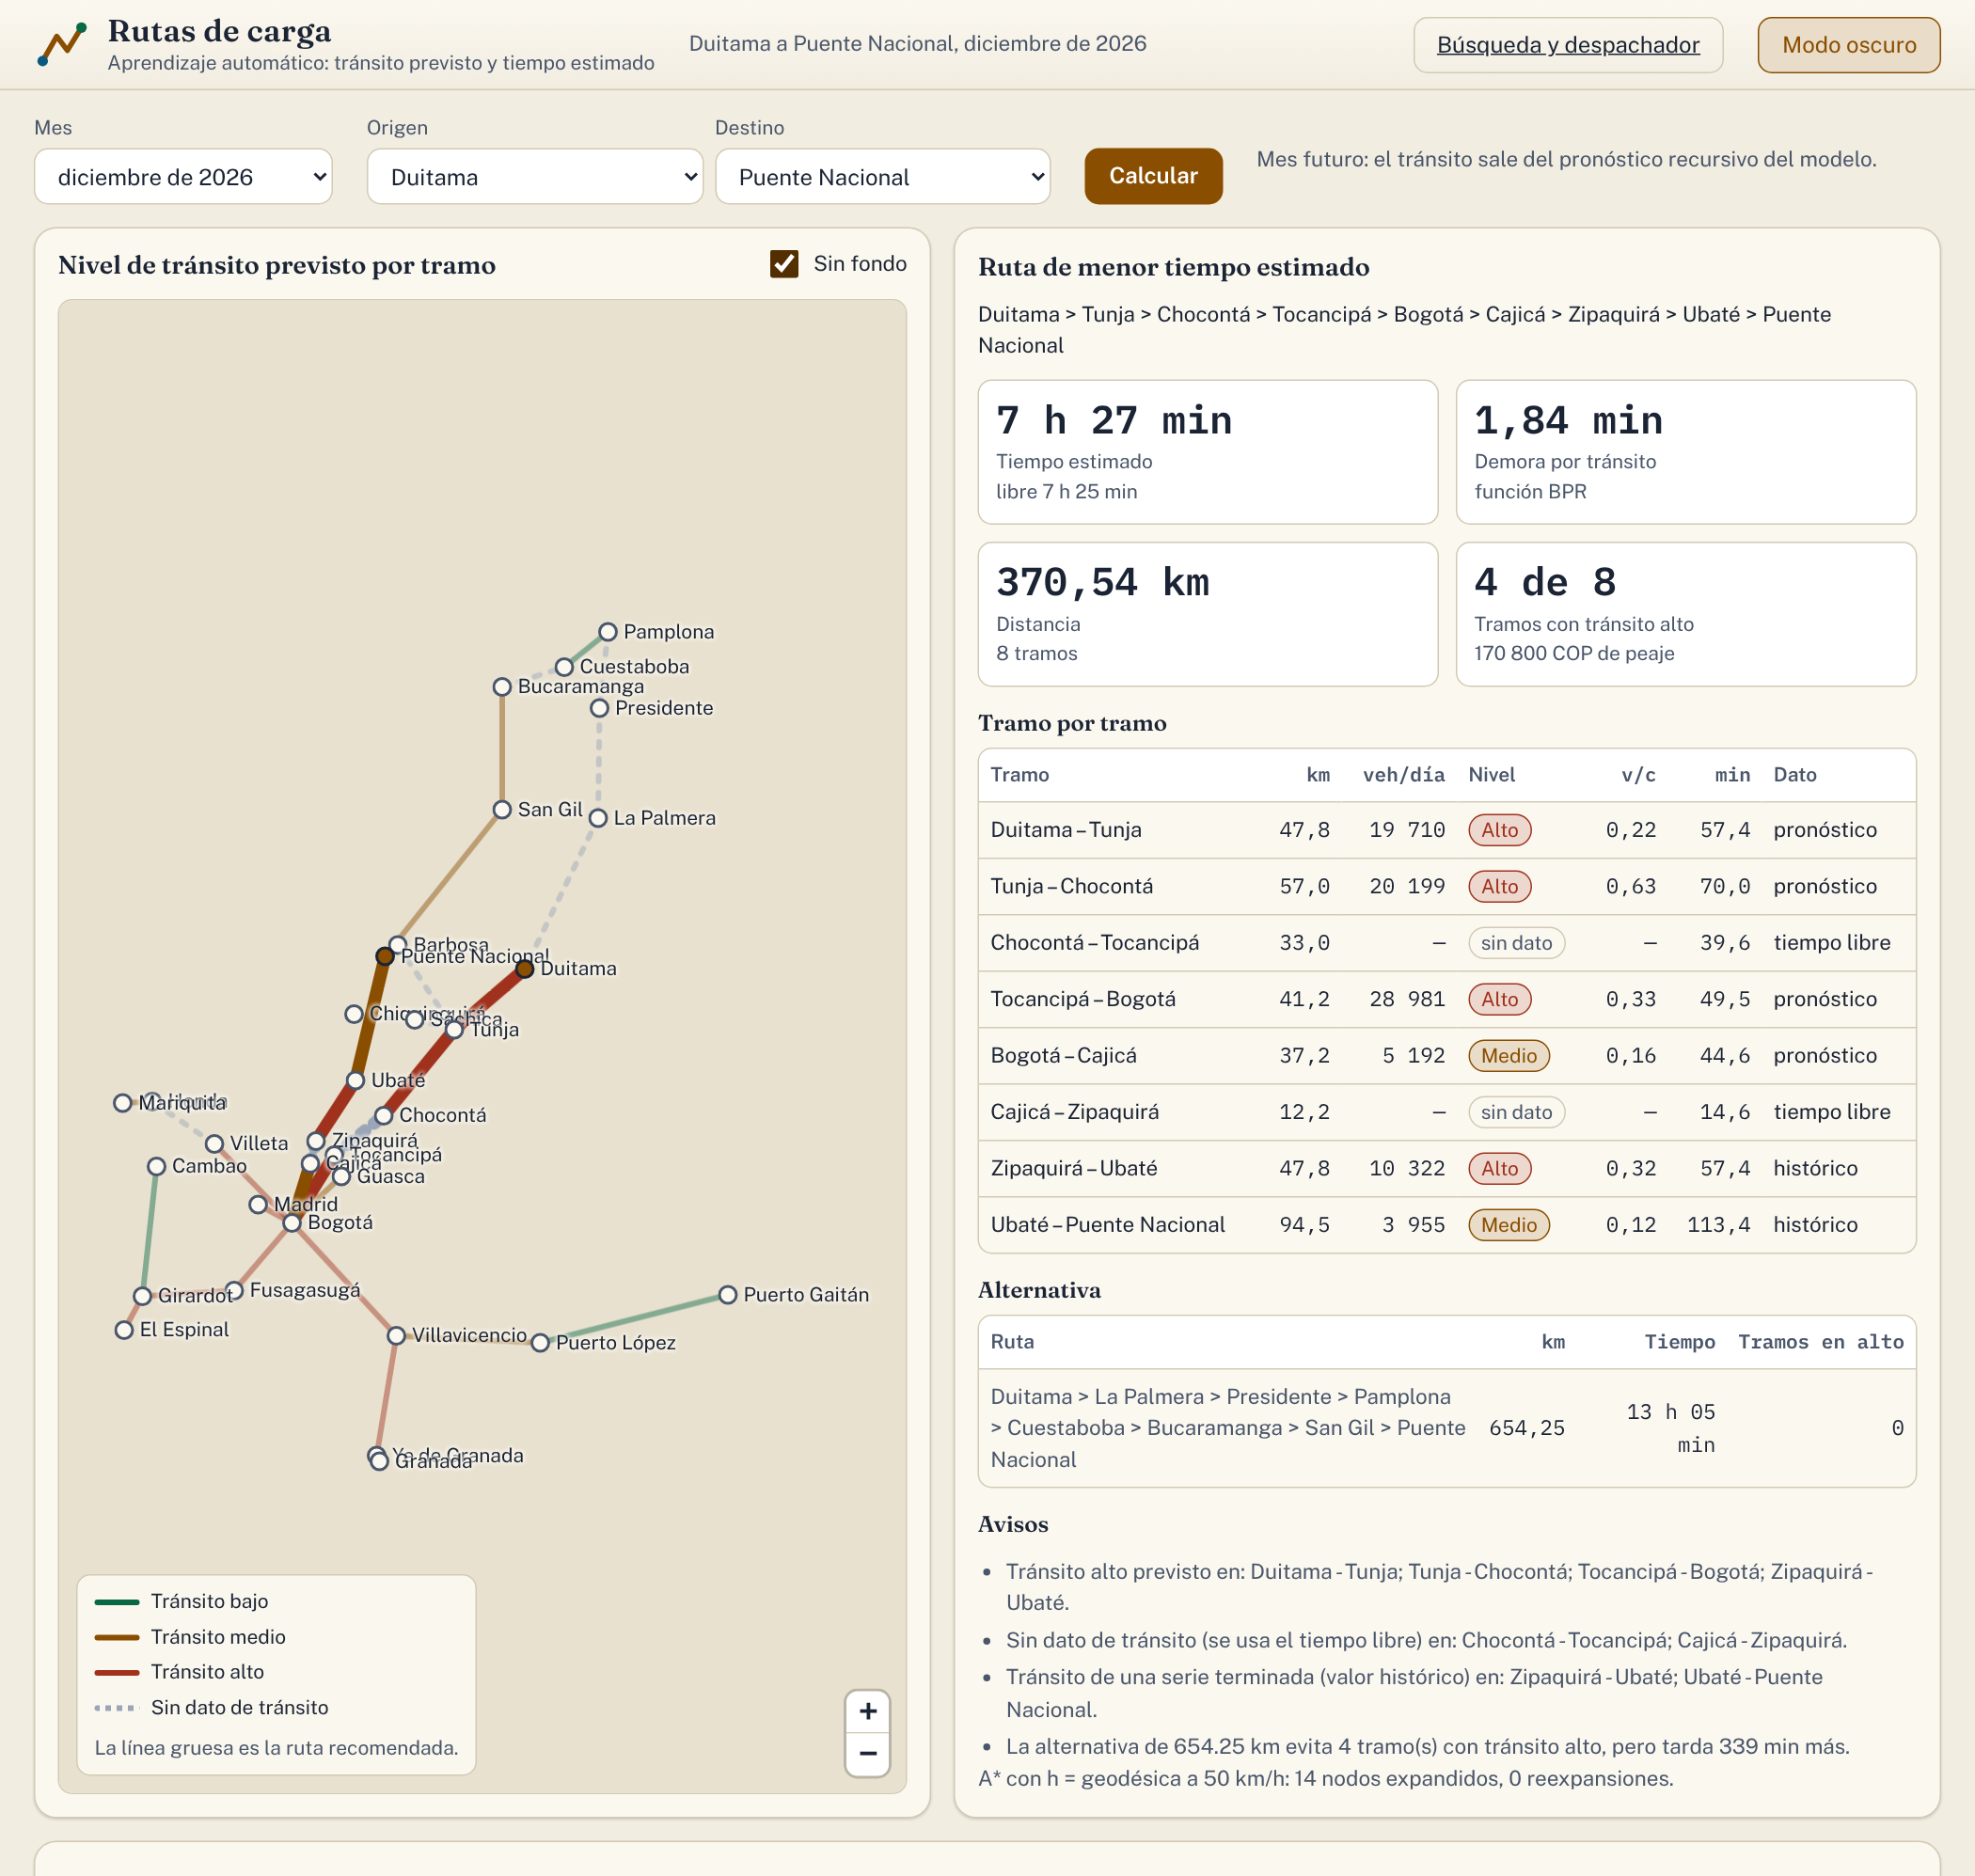
\includegraphics[width=\textwidth]{c3_interfaz.png}
    \caption{Página de aprendizaje automático de la aplicación, caso central. Fuente: elaboración propia}
    \label{fig:interfaz}
    \comoleerla{a la izquierda, el mapa de la red con el nivel previsto de
    cada tramo; a la derecha, la ruta recomendada con sus cifras y su
    detalle.}
    {las mismas cifras de la Tabla~\ref{tab:caso}: \ctCasoKm{} km,
    \ctCasoTiempo{} y \ctCasoAlto{} de \ctCasoTramos{} tramos con tránsito
    alto.}
    {la página no calcula nada: dibuja lo que devuelve el agente
    predictivo.}
\end{figure}

\subsection{Reproducción y pruebas}

\begin{verbatim}
pip install -r requirements.txt
python src/datos_trafico.py
python experimentos/experimentos_corte3.py
python informe/figuras_corte3.py
python informe/tablas_corte3.py
python pruebas/pruebas_corte3.py
python src/agente_predictivo.py Duitama "Puente Nacional" --mes 2026-12
python visualizador/servidor.py
\end{verbatim}

\begin{itemize}
\item \texttt{pruebas/pruebas\_corte3.py} recalcula las métricas desde las
predicciones guardadas, comprueba la partición temporal, la función BPR, la
heurística, la coincidencia de la API con el agente y que cada cifra citada
en este informe sale de \texttt{informe/tablas\_corte3.py}.
\item Las suites de los cortes anteriores siguen pasando: el Corte 3 no
modifica los algoritmos de búsqueda ni los nueve criterios.
\end{itemize}

\section{Limitaciones}
\label{sec:limitaciones}

\begin{itemize}
\item \textbf{El tiempo no es medido.} Sale de una fórmula con cinco
supuestos sin calibrar. Sirve para ordenar rutas, no para prometer una hora
de llegada.
\item \textbf{Promedios mensuales.} La fuente no trae horas ni días. La
saturación de la hora pico se aproxima con un factor fijo; los picos de
puentes festivos y de fines de semana quedan diluidos.
\item \textbf{Nivel de tránsito y congestión.} El nivel mide demanda, no
saturación: un tramo de doble calzada puede estar en nivel alto con
saturación baja.
\item \textbf{Cobertura de la red.} \ctTramosSinDato{} tramos no tienen dato y
\ctTramosHistoricos{} usan una serie terminada. El desvío por Santander no
tiene ningún tramo con serie vigente.
\item \textbf{Un peaje por tramo.} El tránsito medido en el peaje se asigna
al tramo completo.
\item \textbf{Categorías sin diccionario.} El grupo vehicular se deduce del
código de la categoría.
\item \textbf{Pronóstico recursivo.} Su error crece con el horizonte y a
varios meses no supera a la referencia estacional. No anticipa cierres de
peajes.
\item \textbf{Agrupamiento.} La silueta es baja; los grupos describen, no
separan.
\end{itemize}

\section{Conclusiones}
\label{sec:conclusiones}

\begin{enumerate}
\item El proyecto no tenía datos de tiempo ni de congestión. Se resolvió con
un dato real de tránsito (ANI, \ctFilasCrudas{} filas) y una estimación de
tiempo con supuestos declarados, en lugar de datos simulados.
\item La regresión predice el tránsito del mes siguiente con un MAE de
\ctMaeMejor{} vehículos por día, un \ctMejoraMae\,\% menos que la
persistencia. Los cuatro modelos superan a las dos referencias.
\item La clasificación del nivel de tránsito acierta el
\ctExactitudMejor\,\% frente al \ctExactitudPersistencia\,\% de la
persistencia. La ganancia es corta porque el nivel de un corredor es estable.
\item El agrupamiento da \ctKGrupos{} grupos coherentes entre K-medias y el
jerárquico (Rand ajustado de \ctRandAjustado), con silueta baja
(\ctSiluetaKmedias).
\item Con promedios mensuales la saturación máxima es \ctSaturacionMaxima{} y
la demora no pasa de \ctDemoraMaxima{} minutos por tramo. La ruta de menor
tiempo coincide con la de menor distancia; el aporte del aprendizaje al
agente es el nivel de tránsito esperado en cada tramo y sus avisos.
\item La integración reutiliza el A* del Corte 2 con una heurística de tiempo
admisible y consistente, y la aplicación web muestra en una sola página el
pronóstico, la ruta y las métricas de los modelos.
\end{enumerate}

\begin{thebibliography}{9}

\bibitem{formulacion}
Andradé Gómez, J. D., Jiménez López, M., y Díaz García, C. A. (2026).
\textit{Formulación del problema y agente de rutas para una red de carga
interurbana} (Proyecto Integrador, Corte 1) [Documento del equipo].
Universidad Sergio Arboleda.

\bibitem{cortedos}
Andradé Gómez, J. D., Jiménez López, M., y Díaz García, C. A. (2026).
\textit{Algoritmos de búsqueda sobre una red de carga interurbana: BFS, DFS,
costo uniforme, voraz y A*} (Proyecto Integrador, Corte 2) [Documento del
equipo]. Universidad Sergio Arboleda.

\bibitem{ani}
Agencia Nacional de Infraestructura. (2026). \textit{Tráfico Vehicular ANI}.
Datos Abiertos Colombia (descargado el 16 de noviembre de 2026). Licencia
CC BY-SA 4.0. \url{https://www.datos.gov.co/resource/8yi9-t44c}

\bibitem{bpr}
Bureau of Public Roads. (1964). \textit{Traffic Assignment Manual}. U.S.
Department of Commerce, Urban Planning Division.

\bibitem{sklearn}
Pedregosa, F., Varoquaux, G., Gramfort, A., Michel, V., Thirion, B., Grisel,
O., y otros. (2011). Scikit-learn: Machine learning in Python. \textit{Journal
of Machine Learning Research, 12}, 2825--2830.

\end{thebibliography}

\end{document}
